\documentclass[journal,12pt,onecolumn]{IEEEtran}
\usepackage{cite}
\usepackage{amsmath,amssymb,amsfonts,amsthm}
\usepackage{algorithmic}
\usepackage{graphicx}
\graphicspath{{./figs/}}
\usepackage{textcomp}
\usepackage{xcolor}
\usepackage{txfonts}
\usepackage{listings}
\usepackage{enumitem}
\usepackage{mathtools}
\usepackage{gensymb}
\usepackage{comment}
\usepackage{caption}
\usepackage[breaklinks=true]{hyperref}
\usepackage{tkz-euclide} 
\usepackage{listings}
\usepackage{gvv}                                           
\usepackage{xparse}
\usepackage{color}                                            
\usepackage{array}                                            
\usepackage{longtable}                                       
\usepackage{calc}                                             
\usepackage{multirow}
\usepackage{multicol}
\usepackage{hhline}                                           
\usepackage{ifthen}                                           
\usepackage{lscape}
\usepackage{tabularx}
\usepackage{array}
\usepackage{float}
\usepackage[margin=1in]{geometry}
\usepackage{fancyhdr}
\usepackage{chemfig}
\usepackage{multicol}
 \usepackage{amsmath}
\usepackage{enumitem}
\usepackage{array}
\usepackage{titlesec}
\usepackage{tabularx} 
\usepackage{amsmath, amssymb}
\usepackage{extarrows}
\usepackage{chemarr}
\usepackage[utf8]{inputenc}
\usepackage{chemmacros} 
\usepackage{graphicx}
\chemsetup{modules={reactions}} 

\pagestyle{fancy}
\fancyhf{}
\fancyhead[L]{\textit{2016}}
\fancyhead[R]{\textbf{GATE XL}}
\renewcommand{\headrulewidth}{0.4pt}

\begin{document}

\section*{\centering GA : GENERAL APTITUDE (Compulsory)}
\noindent \textbf{ 1 --  5 carry one mark each.}
\begin{enumerate}[label=\arabic*.]

\item The chairman requested the aggrieved shareholders to \rule{3cm}{0.1pt} him.
\begin{multicols}{4}
\begin{enumerate}[label=(\Alph*)]
\item bare with
\item bore with
\item bear with
\item bare
\end{enumerate}
\end{multicols}

\item Identify the correct spelling out of the given options:
\begin{multicols}{4}
\begin{enumerate}[label=(\Alph*)]
\item Managable
\item Manageable
\item Mangaeble
\item Managible
\end{enumerate}
\end{multicols}

\item Pick the odd one out in the following: 13, 23, 33, 43, 53
\begin{multicols}{4}
\begin{enumerate}[label=(\Alph*)]
\item 23
\item 33
\item 43
\item 53
\end{enumerate}
\end{multicols}

\item R2D2 is a robot. R2D2 can repair aeroplanes. No other robot can repair aeroplanes.\\
Which of the following can be logically inferred from the above statements?
\begin{multicols}{2}
\begin{enumerate}[label=(\Alph*)]
\item R2D2 is a robot which can only repair aeroplanes.
\item R2D2 is the only robot which can repair aeroplanes.
\item R2D2 is a robot which can repair only aeroplanes.
\item Only R2D2 is a robot.
\end{enumerate}
\end{multicols}

\item If $|9y-6|=3$, then $y^2 -\frac{4y}{3}$ is \rule{2.5cm}{0.1pt}.
\begin{multicols}{4}
\begin{enumerate}[label=(\Alph*)]
\item 0
\item $+\frac{1}{3}$
\item $-\frac{1}{3}$
\item undefined
\end{enumerate}
\end{multicols}

\noindent \textbf{ 6 --  10 carry two marks each.}

\item The following graph represents the installed capacity for cement production (in tonnes) and the actual production (in tonnes) of nine cement plants of a cement company. Capacity utilization of a plant is defined as ratio of actual production of cement to installed capacity. A plant with installed capacity of at least 200 tonnes is called a large plant and a plant with lesser capacity is called a small plant. The difference between total production of large plants and small plants, in tonnes is \rule{3cm}{0.1pt}.

\begin{figure}[H]
    \centering
    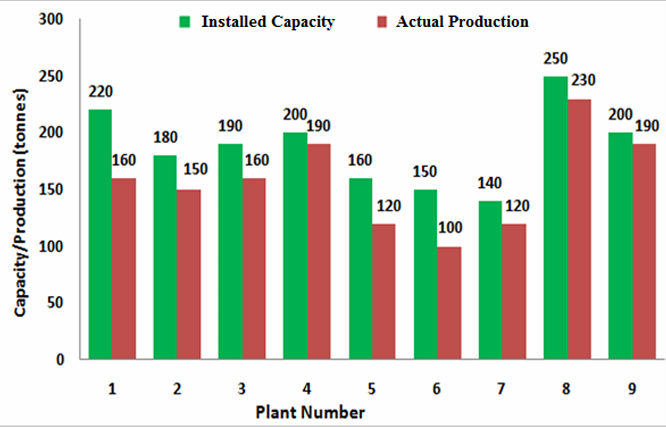
\includegraphics[width=0.7\columnwidth]{FIG/GA-6.png}
    \caption*{}
    \label{fig:GA-6}
\end{figure}

\item A poll of students appearing for masters in engineering indicated that 60\% of the students believed that mechanical engineering is a profession unsuitable for women. A research study on women with masters or higher degrees in mechanical engineering found that 99\% of such women were successful in their professions.

Which of the following can be logically inferred from the above paragraph?
\begin{enumerate}[label=(\Alph*)]
\item Many students have misconceptions regarding various engineering disciplines.
\item Men with advanced degrees in mechanical engineering believe women are well suited to be mechanical engineers.
\item Mechanical engineering is a profession well suited for women with masters or higher degrees in mechanical engineering.
\item The number of women pursuing higher degrees in mechanical engineering is small.
\end{enumerate}

\item Sourya committee had proposed the establishment of Sourya Institutes of Technology (SITs) in line with Indian Institutes of Technology (IITs) to cater to the technological and industrial needs of a developing country.
Which of the following can be logically inferred from the above sentence?
Based on the proposal,
\begin{enumerate}[label=(\roman*)]
\item In the initial years, SIT students will get degrees from IIT.
\item SITs will have a distinct national objective.
\item SIT like institutions can only be established in consultation with IIT.
\item SITs will serve technological needs of a developing country.
\end{enumerate}
\vspace{-2ex}
\begin{multicols}{2}
\begin{enumerate}[label=(\Alph*)]
\item (iii) and (iv) only.
\item (i) and (iv) only.
\item (ii) and (iv) only.
\item (ii) and (iii) only.
\end{enumerate}
\end{multicols}

\item Shaquille O’Neal is a 60\% career free throw shooter, meaning that he successfully makes 60 free throws out of 100 attempts on average. What is the probability that he will successfully make exactly 6 free throws in 10 attempts?
\begin{multicols}{4}
\begin{enumerate}[label=(\Alph*)]
\item 0.2508
\item 0.2816
\item 0.2934
\item 0.6000
\end{enumerate}
\end{multicols}

\item The numeral in the units position of $2^{11870} + 14^{6127}\times34^{24}$ is \rule{2.5cm}{0.1pt}.
\end{enumerate}
\begin{center}
\textbf{END OF QUESTION PAPER}
\end{center}
\newpage
\section*{\centering H : CHEMISTRY (Compulsory)}
\noindent \textbf{ 1 --  5 carry one mark each.}
\begin{enumerate}[label=\arabic*.]

\item The species having shortest B‒F bond distance is
\begin{multicols}{4}
\begin{enumerate}[label=(\Alph*)]
\item BF$_3$
\item [BF$_4$]$^-$
\item H$_3$N$\cdot$BF$_3$
\item (CH$_3$)$_2$O$\cdot$BF$_3$
\end{enumerate}
\end{multicols}

\item The total number of chair conformations possible for 1,2-dimethylcyclohexane is \rule{2.5cm}{0.1pt}.

\item ‘A harmful substance persists in the environment for a very long period of time’. The UNACCEPTABLE statement for this fact is
\begin{enumerate}[label=(\Alph*)]
\item the substance degrades by second-order kinetics
\item the substance degrades by first-order kinetics
\item the substance is not biodegradable
\item the substance has long half-life
\end{enumerate}

\item For an enzyme catalyzed reaction, the plot that correctly represents the relationship between the rate and temperature is

\begin{figure}[H]
    \centering
    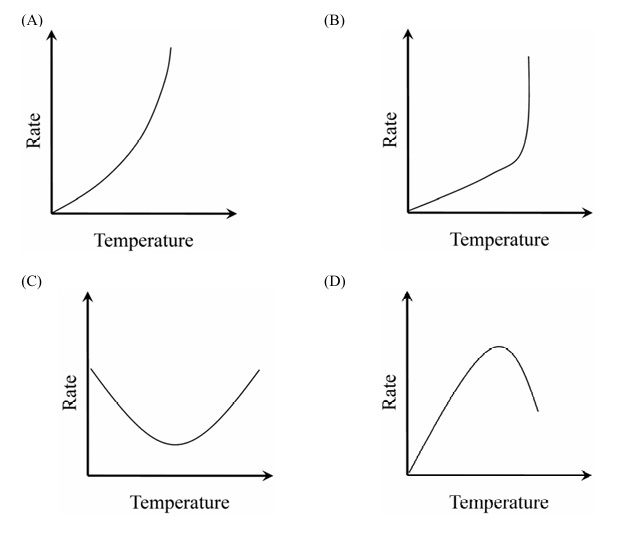
\includegraphics[width=0.7\columnwidth]{FIG/H-4.png}
    \caption*{}
    \label{fig:H-4}
\end{figure}

\item Combinations of a process and equation are given below. The INCORRECT combination is
\begin{enumerate}[label=(\Alph*)]
\item Constant pressure heating with no phase change; $q = nC_P\Delta T$
\item Reversible adiabatic process in a perfect gas; $\Delta S = nC_V\ln\frac{T_2}{T_1}$
\item Reversible isothermal process in a perfect gas; $q_{\text{rev}} = -nRT\ln\frac{V_2}{V_1}$
\item Constant volume heating with no phase change; $\Delta U = nC_V\Delta T$
\end{enumerate}

\noindent \textbf{ 6 --  15 carry two marks each.}

\item The correct comparison of pK$_a$’s of [Fe(H$_2$O)$_6$]$^{2+}$, [Fe(H$_2$O)$_6$]$^{3+}$, V$_2$O$_5$ and N$_2$O$_5$ is
\begin{enumerate}[label=(\Alph*)]
\item[(A)] [Fe(H$_2$O)$_6$]$^{3+}$ $<$ [Fe(H$_2$O)$_6$]$^{2+}$ and V$_2$O$_5$ $<$ N$_2$O$_5$
\item[(B)] [Fe(H$_2$O)$_6$]$^{3+}$ $<$ [Fe(H$_2$O)$_6$]$^{2+}$ and V$_2$O$_5$ = N$_2$O$_5$
\item[(C)] [Fe(H$_2$O)$_6$]$^{2+}$ = [Fe(H$_2$O)$_6$]$^{3+}$ and N$_2$O$_5$ $<$ V$_2$O$_5$
\item[(D)] [Fe(H$_2$O)$_6$]$^{3+}$ $<$ [Fe(H$_2$O)$_6$]$^{2+}$ and N$_2$O$_5$ $<$ V$_2$O$_5$
\end{enumerate}

\item Given: The potential energy of two electrons separated by Bohr radius is 27.211 eV. The first Bohr radius of hydrogen is 0.5292 \AA. The electron makes an orbit of radius 0.5295 \AA\ around the nucleus in hydrogen.  The calculated ionization energy (eV) of hydrogen atom is \rule{2.5cm}{0.1pt}.

\item The crystal field stabilization energy (excluding pairing energy, if any) of [CoCl$_4$]$^{2-}$ in $\Delta_o$ units is \rule{2.5cm}{0.1pt}.

\item The correct statement is
\begin{enumerate}[label=(\Alph*)]
\item TlBr$_3$ is less soluble in water than TlBr
\item Ag$_2$S is more soluble in water than Ag$_2$O
\item LiF is less stable than CsF
\item [(D)][Co(NH$_3$)$_5$I]$^{2+}$ is less stable than [Co(NH$_3$)$_5$F]$^{2+}$
\end{enumerate}

\item Ferrous sulfate on reaction with potassium hexacyanochromate(III) produces a brick red complex. The number of unpaired electrons on Fe in the red complex is \rule{2.5cm}{0.1pt}.

\item The major product formed in the following reaction is (ignore product stereochemistry)

\({\chemfig{*6(---(--[::300]COOH)-=-)}} 
{\overset{\text{$I_2$,NAHCO$_3$}}{\longrightarrow}} 
\)

\begin{figure}[H]
    \centering
    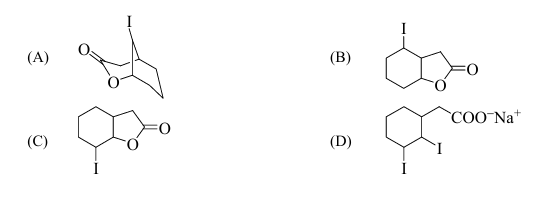
\includegraphics[width=0.9\columnwidth]{FIG/H-11.png}
    \caption*{}
    \label{fig:H-11}
\end{figure}

\item When 1.0 g of urea (Molecular Weight = 60) is dissolved in 200 g of solvent S, the freezing point of S is lowered by 0.25 $^\circ$C. When 1.5 g of a non-electrolyte Y is dissolved in 125 g of S, the freezing point of S is lowered by 0.20 $^\circ$C. The molecular weight of Y is \rule{2.5cm}{0.1pt}.

\item The major product formed in the following reaction is\\
\[
{\chemfig{*5(---=(-CH_3)-)}}
\xrightarrow{\text{(i) B}_2\text{H}_6,\ \text{diglyme}\hspace{1em} \text{(ii) H}_2\text{O}_2,\ \text{HO}^-}
\]
\begin{figure}[H]
    \centering
    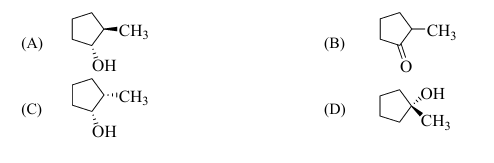
\includegraphics[width=0.9\columnwidth]{FIG/H-13.png}
    \caption*{}
    \label{fig:H-13}
\end{figure}
\item For a weak acid at 298 K the molar conductivities (in ohm$^{-1}$ m$^2$ mol$^{-1}$), at infinite dilution and 0.04 mol dm$^{-3}$ are $4.3 \times 10^{-3}$ and $1.0 \times 10^{-3}$, respectively. The degree of dissociation of the acid (0.04 mol dm$^{-3}$) at 298 K is \rule{2.5cm}{0.1pt}.

\item For propene at 298 K, the molar enthalpy of hydrogenation is $-124.27$ kJ mol$^{-1}$ and the standard enthalpy of formation is $20.42$ kJ mol$^{-1}$. For propane at 298 K, the standard enthalpy of formation in kJ mol$^{-1}$ is \rule{2.5cm}{0.1pt}.
\end{enumerate}
\begin{center}
\textbf{END OF QUESTION PAPER}
\end{center}
\newpage
\section*{\centering I : BIOCHEMISTRY}

\noindent \textbf{ 1 -- 10 carry one mark each.}

\begin{enumerate}[label=\arabic*.]

\item Heterologous expression of green fluorescent protein is possible because the genetic code is

\begin{multicols}{4}
\begin{enumerate}[label=(\Alph*)]
\item universal
\item triplet
\item degenerate
\item non-overlapping
\end{enumerate}
\end{multicols}

\item Phosphoglucose isomerase was incubated with 0.2 M of glucose 6-phosphate.
On reaching equilibrium, 55\% of glucose 6-phosphate was converted to fructose 6-phosphate. The equilibrium constant for this reaction is \rule{2.5cm}{0.1pt}.

\item Hydrolysis of a peptide involves cleavage of the bond between the atoms

\begin{multicols}{4}
\begin{enumerate}[label=(\Alph*)]
\item N and C$\alpha$
\item C and O
\item C$\alpha$ and C
\item N and C
\end{enumerate}
\end{multicols}

\item Inter-conversion of UDP-glucose and UDP-galactose is catalyzed by

\begin{multicols}{4}
\begin{enumerate}[label=(\Alph*)]
\item an oxidase
\item a kinase
\item an epimerase
\item a mutase
\end{enumerate}
\end{multicols}

\item Gel filtration profile and corresponding activity data for a pure enzyme are shown in the figure below. The same enzyme sample on SDS-PAGE runs as a 30 kDa polypeptide.

\begin{figure}[H]
\centering
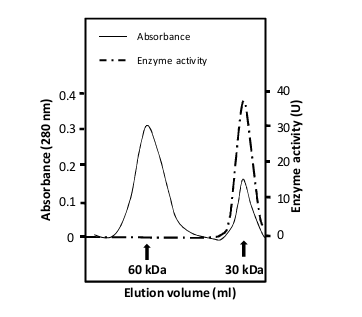
\includegraphics[width=0.7\columnwidth]{FIG/I-5.png}
\caption*{}
\label{fig:I-5}
\end{figure}

Which one of the following is the correct interpretation of the data?

\begin{multicols}{2}
\begin{enumerate}[label=(\Alph*)]
\item Both monomer and dimer are active
\item Enzyme is active only as a monomer
\item Protein does not form dimers
\item Enzyme is active only as a dimer
\end{enumerate}
\end{multicols}

\item Amino acid residues predominantly involved in protein-DNA interactions are

\begin{multicols}{4}
\begin{enumerate}[label=(\Alph*)]
\item alanines
\item negatively charged
\item prolines
\item positively charged
\end{enumerate}
\end{multicols}

\item Cellulose serves as a structural polymer whereas starch does not. This is because cellulose contains

\begin{enumerate}[label=(\Alph*)]
\item $\beta$1$\rightarrow$4 linked glucose monomers and inter-chain hydrogen bonds
\item $\beta$1$\rightarrow$4 linked glucose monomers and intra-chain hydrogen bonds
\item $\alpha$1$\rightarrow$4 linked glucose monomers and inter-chain hydrogen bonds
\item $\alpha$1$\rightarrow$4 linked glucose monomers and intra-chain hydrogen bonds
\end{enumerate}

\item Molar absorption spectra labeled (i), (ii) and (iii) for three different amino acids are shown below.

 \begin{figure}[H]
 \centering
 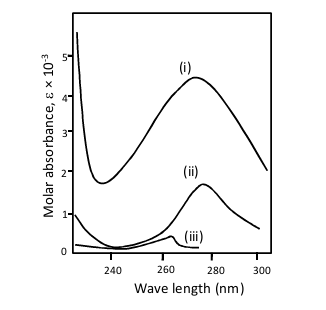
\includegraphics[width=0.7\columnwidth]{FIG/I-8.png}
 \caption*{}
 \label{fig:I-8}
 \end{figure}

Which one of the following is the correct combination of spectral assignments?

\begin{enumerate}[label=(\Alph*)]
\item (i) - tryptophan, (ii) - tyrosine, (iii) - phenylalanine
\item (i) - phenylalanine, (ii) - tryptophan, (iii) - tyrosine
\item (i) - proline, (ii) - tyrosine, (iii) - tryptophan
\item (i) - tryptophan, (ii) - proline, (iii) - phenylalanine
\end{enumerate}

\item The fluidity of a phospholipid membrane increases when the fatty acid

\begin{enumerate}[label=(\Alph*)]
\item chain length increases and degree of unsaturation decreases
\item chain length decreases and degree of unsaturation increases
\item chain length decreases and degree of unsaturation decreases
\item chain length increases and degree of unsaturation increases
\end{enumerate}

\item Polypeptides are biosynthesized on the ribosomes inside the cell. Chemical synthesis of polypeptides is also possible through Merrifield’s solid-phase peptide synthesis. In both the cases the polypeptide chain is extended one amino acid at a time. The direction of polypeptide synthesis is from

\begin{enumerate}[label=(\Alph*)]
\item C-terminus to N-terminus in both the cases
\item N-terminus to C-terminus in both the cases
\item C-terminus to N-terminus on the ribosomes and N-terminus to C-terminus in solid-phase synthesis
\item N-terminus to C-terminus on the ribosomes and C-terminus to N-terminus in solid-phase synthesis
\end{enumerate}

\end{enumerate}

\vspace{0.5cm}
\noindent \textbf{ 11 -- 20 carry two marks each.}

\begin{enumerate}[label=\arabic*.,resume]

\item Four groups of metabolites are given below. Choose the group in which all the compounds contain at least one bond whose $\Delta G'^{o}$ of hydrolysis is $\leq -7.0$ kcal/mole.

\begin{enumerate}[label=(\Alph*)]
\item Glucose 1-phosphate, Adenosine triphosphate, Fructose 1,6-bisphosphate
\item Creatine phosphate, Acetyl phosphate, Succinyl CoA
\item Glycerol 3-phosphate, Acetyl CoA, 1,3-Bisphosphoglycerate
\item Glucose 6-phosphate, Phosphoenolpyruvate, Adenosine diphosphate
\end{enumerate}

\item The $\Delta G'^{o}$ for the malate dehydrogenase catalyzed step of Krebs cycle is $+7.1$ kcal/mole. Nevertheless, the conversion of malate to oxaloacetate in vivo proceeds spontaneously because the subsequent reaction that consumes oxaloacetate has a $\Delta G'^{o}$ of \rule{2.5cm}{0.1pt}.

\begin{multicols}{2}
\begin{enumerate}[label=(\Alph*)]
\item $-3.0$ kcal/mole
\item $+3.0$ kcal/mole
\item $-7.7$ kcal/mole
\item $+7.7$ kcal/mole
\end{enumerate}
\end{multicols}

\item When freshly isolated intact mitochondria were incubated with ADP and inorganic phosphate neither the oxygen consumption nor the ATP synthesis could be detected. Addition of succinate resulted in increased oxygen consumption as well as ATP synthesis with time. Subsequent addition of cyanide to this system will result in which one of the following?

\begin{enumerate}[label=(\Alph*)]
\item Both oxygen consumption and ATP synthesis are inhibited
\item Oxygen consumption continues but ATP synthesis is inhibited
\item Oxygen consumption is inhibited but ATP synthesis continues
\item Both oxygen consumption and ATP synthesis continue
\end{enumerate}

\item Three micrograms of a circular plasmid of 4200 bp was digested with a restriction enzyme and subjected to agarose gel electrophoresis. Five DNA fragments of different sizes were observed and their sizes summed up to 4200 bp. The number of picomoles of DNA ends generated after complete digestion with the enzyme is \rule{2.5cm}{0.1pt}.

\item An enzyme was purified using ion-exchange chromatography and the results are shown in the table below.\\

\begin{tabular}{|c|c|c|c|}
\hline
Step & Volume (ml) & Total protein (mg) & Total activity (U) \\
\hline
Cell extract & 8000 & 400 & 800 \\
DEAE Sephacel 10 & 2 & 200 & \\
\hline
\end{tabular}\\

Which one of the following is the correct interpretation of these data?

\begin{enumerate}[label=(\Alph*)]
\item 50 fold purification was achieved with 25\% yield of the enzyme
\item 25 fold purification was achieved with 50\% yield of the enzyme
\item 50 fold purification was achieved with 4\% yield of the enzyme
\item 200 fold purification was achieved with 25\% yield of the enzyme
\end{enumerate}

\item Aspartate residues are found in the active sites of many enzymes. The pK$_a$ for the $\beta$-carboxylate of aspartate is 3.86. At physiological pH this group can function as

\begin{multicols}{2}
\begin{enumerate}[label=(\Alph*)]
\item a nucleophile and a conjugate acid
\item an electrophile and a conjugate acid
\item a nucleophile and a conjugate base
\item an electrophile and a conjugate base
\end{enumerate}
\end{multicols}

\item Kinetic parameters for the enzyme fumarase with three different substrates are given below.\\
\begin{center}
\begin{tabular}{|c|c|c|}
\hline
Substrate & $K_M$ ($\mu$M) & $k_{cat}$ (sec$^{-1}$) \\
\hline
Fluorofumarate & 27 & 2700 \\
Fumarate & 5 & 800 \\
Chlorofumarate & 111 & 20 \\
\hline
\end{tabular}\\
\end{center}

The specificity of fumarase for the substrates decreases in the order

\begin{enumerate}[label=(\Alph*)]
\item Fluorofumarate $>$ Fumarate $>$ Chlorofumarate
\item Chlorofumarate $>$ Fluorofumarate $>$ Fumarate
\item Fumarate $>$ Fluorofumarate $>$ Chlorofumarate
\item Fumarate $>$ Chlorofumarate $>$ Fluorofumarate
\end{enumerate}

\item A polypeptide with the amino acid sequence ‘AGKPDHEKAHL’ was dissolved in a buffer of pH 1.8. The predominant form of the polypeptide will have a net charge of

\begin{multicols}{4}
\begin{enumerate}[label=(\Alph*)]
\item $+4$
\item $+5$
\item $+7$
\item $+11$
\end{enumerate}
\end{multicols}

\item An N-terminal His-tagged protein of molecular weight 40 kDa was purified using Ni-NTA column. This protein sample was subjected to SDS-PAGE. A western blot of the same using anti-His antibodies is shown below.

\begin{figure}[H]
\centering
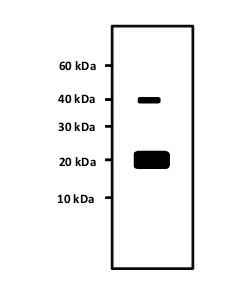
\includegraphics[width=0.7\columnwidth]{FIG/I-19.png}
\caption*{}
\label{fig:I-19}
\end{figure}

Which one of the following interpretations is correct?

\begin{enumerate}[label=(\Alph*)]
\item Only the His-tag of the protein got removed
\item The protein forms oligomers
\item The purified protein sample is homogeneous
\item The protein has a stable N-terminal 20 kDa domain
\end{enumerate}

\item The sequence of a polypeptide that forms a transmembrane helix is shown below.

\begin{verbatim}
TGERVQLAHH FSEPEITLII FGVMAGVIGT ILLASYGIRR LIKKSP
1          11        21         31         41
\end{verbatim}


Which one of the following segments of the peptide is most likely to span the membrane?

\begin{multicols}{2}
\begin{enumerate}[label=(\Alph*)]
\item E3-G22
\item V5-A25
\item E15-A34
\item F21-R40
\end{enumerate}
\end{multicols}

\end{enumerate}

\begin{center}
\textbf{END OF QUESTION PAPER}
\end{center}
\newpage
\section*{\centering J : BOTANY}

\noindent \textbf{ 1 -- 10 carry one mark each.}

\begin{enumerate}[label=\arabic*.]

\item Which of the following is most abundant in the aleurone layer of wheat seeds?

\begin{multicols}{4}
\begin{enumerate}[label=(\Alph*)]
\item Tannin
\item Starch
\item Protein
\item Lipid
\end{enumerate}
\end{multicols}

\item Which of the following does NOT use xylem to transport water?

\begin{multicols}{4}
\begin{enumerate}[label=(\Alph*)]
\item Miscanthus
\item Marchantia
\item Selaginella
\item Magnolia
\end{enumerate}
\end{multicols}

\item Which of the following is the closest ancestor of all land plants?

\begin{multicols}{4}
\begin{enumerate}[label=(\Alph*)]
\item Blue green algae
\item Red algae
\item Chara
\item Coleochaeteae
\end{enumerate}
\end{multicols}

\item 4',6-diamidino 2-phenylindole (DAPI) is a fluorescent dye used to stain the nucleus. Which of the following plant cells, when mature, cannot be stained by DAPI?

\begin{multicols}{4}
\begin{enumerate}[label=(\Alph*)]
\item Trichomes
\item Tracheids
\item Collenchyma
\item Mesophyll
\end{enumerate}
\end{multicols}

\item The uptake of nitrogen (N) and phosphorus (P) by plant roots often involves interaction between root and some symbiotic organisms. Which of the following associations is most commonly found for the uptake of these two nutrients?

\begin{multicols}{2}
\begin{enumerate}[label=(\Alph*)]
\item Bacteria for N, algae for P
\item Bacteria for N, nematodes for P
\item Nematodes for N, fungi for P
\item Bacteria for N, mycorrhizae for P
\end{enumerate}
\end{multicols}

\item Which of the following summarizes the role of Casparian strip in transport of water in the root?

\begin{multicols}{2}
\begin{enumerate}[label=(\Alph*)]
\item Symplast to Apoplast
\item Apoplast to Symplast
\item Phloem to Xylem
\item Xylem to Phloem
\end{enumerate}
\end{multicols}

\item Atropine is a drug used in the management of pesticide poisoning. Which of the following plants can serve as a commercial source of this anticholinergic drug?

\begin{multicols}{2}
\begin{enumerate}[label=(\Alph*)]
\item Datura metel
\item Medicago trancatula
\item Mangifera indica
\item Arachis hypogaea
\end{enumerate}
\end{multicols}

\item Which of the following is NOT involved in plant immune response?

\begin{multicols}{2}
\begin{enumerate}[label=(\Alph*)]
\item Antimicrobial proteins
\item Hypersensitive response
\item Pattern recognition receptors
\item Interleukins
\end{enumerate}
\end{multicols}

\item Which of the following is a neutral phenomenon?

\begin{multicols}{2}
\begin{enumerate}[label=(\Alph*)]
\item Natural selection
\item Sexual selection
\item Genetic drift
\item Population bottleneck
\end{enumerate}
\end{multicols}

\item When a plant is infected by a pathogen at one site, the distal parts of the plant and neighboring plants develop increased resistance to subsequent pathogen attack. Which of the following molecules mediates this long-distance signal?

\begin{multicols}{2}
\begin{enumerate}[label=(\Alph*)]
\item Nitric oxide
\item Ethylene
\item Jasmonic acid and its derivatives
\item Salicylic acid and its derivatives
\end{enumerate}
\end{multicols}

\end{enumerate}

\vspace{0.5cm}
\noindent \textbf{ 11 -- 20 carry two marks each.}

\begin{enumerate}[label=\arabic*.,resume]

\item An inbred line of a plant with red flower and tall stem was crossed to another inbred line with white flower and short stem. The F$_1$ plants, which all had red flower and tall stem, were backcrossed to the line with white flower and short stem, and the following F$_2$ individuals were obtained: 103 red, tall; 89 white, short; 26 red, short; and 23 white, tall. What is the recombination percentage between the flower color locus and the stem height locus?

\begin{multicols}{2}
\begin{enumerate}[label=(\Alph*)]
\item 19-21\%
\item 49-51\%
\item 79-81\%
\item 0-2\%
\end{enumerate}
\end{multicols}

\item Consider the following pathway controlling time to flowering in wheat:
\begin{figure}[H]
\centering
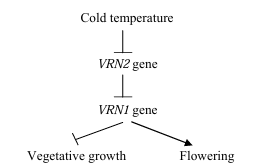
\includegraphics[width=0.7\columnwidth]{FIG/J-12.png}
\caption*{}
\label{fig:J-12}
\end{figure}

If batch P of wheat seed is vernalized before sowing and batch Q is not vernalized, then which of the following statements is most likely to be correct?

\begin{enumerate}[label=(\Alph*)]
\item P will have lower VRN2 transcript and will flower later than Q
\item P will have lower VRN2 transcript and will flower earlier than Q
\item P will have higher VRN2 transcript and will flower later than Q
\item P and Q will have equal VRN2 transcript and will flower at the same time
\end{enumerate}

\item The three plots P, Q and R (in different units) in the graph below represent the dependence of photosynthesis rate (PR), leaf expansion rate (LER) and translocation rate of assimilates (TR) in a plant on leaf water potential. Which of the following statements is correct in this regard?

\begin{figure}[H]
\centering
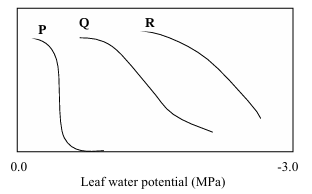
\includegraphics[width=0.7\columnwidth]{FIG/J-13.png}
\caption*{}
\label{fig:J-13}
\end{figure}

\begin{enumerate}[label=(\Alph*)]
\item P represents LER; Q represents TR; R represents PR
\item P represents TR; Q represents PR; R represents LER
\item P represents PR; Q represents LER; R represents TR
\item P represents LER; Q represents PR; R represents TR
\end{enumerate}

\item PIN proteins are plasma membrane-localized carrier proteins required for polar auxin transport in plants. Four different carrier proteins are shown in the diagram below labeled P1-P4. Arrow indicates the direction of auxin flow. Which among these is most likely to be a PIN protein?

\begin{figure}[H]
\centering
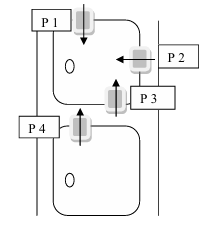
\includegraphics[width=0.6\columnwidth]{FIG/J-14.png}
\caption*{}
\label{fig:J-14}
\end{figure}

\begin{multicols}{2}
\begin{enumerate}[label=(\Alph*)]
\item P1
\item P2
\item P3
\item P4
\end{enumerate}
\end{multicols}

\item An RFLP marker shows sequence polymorphism in two ecotypes (X and Y) of a plant. In ecotype X, the marker contains one GAATTC site in its sequence, whereas in Y it has the sequence GAAATC at the same site. The rest of the sequence is identical in both ecotypes. In a genotyping experiment, the marker was PCR amplified from four different seedlings (P, Q, R, S), completely digested with EcoRI and the products were analyzed by electrophoresis. The diagram below shows the band patterns obtained. Based on the information provided, which of the following statements is correct?

\begin{figure}[H]
\centering
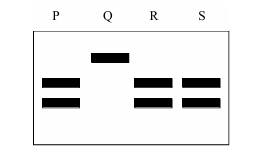
\includegraphics[width=0.6\columnwidth]{FIG/J-15.png}
\caption*{}
\label{fig:J-15}
\end{figure}

\begin{multicols}{2}
\begin{enumerate}[label=(\Alph*)]
\item Seedling Q belongs to ecotype Y
\item Seedling Q belongs to ecotype X
\item Seedling P belongs to ecotype Y
\item Seedling R belongs to ecotype Y
\end{enumerate}
\end{multicols}

\item The cell surface expands differently in different plant cells. Two common modes of expansion are shown below (X and Y). Each rectangular box represents a cell marked with dots on its surface. The spacing between the dots changes after the cell has undergone expansion as indicated by the arrow. Which of the following statements is correct with respect to the growth of root hair and pollen tube?

\begin{figure}[H]
\centering
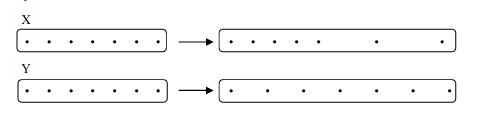
\includegraphics[width=0.7\columnwidth]{FIG/J-16.png}
\caption*{}
\label{fig:J-16}
\end{figure}

\begin{enumerate}[label=(\Alph*)]
\item Both grow as shown in X
\item Both grow as shown in Y
\item Pollen tube grows as shown in X, root hair grows as shown in Y
\item Root hair grows as shown in X, pollen tube grows as shown in Y
\end{enumerate}

\item Hardy Weinberg's equilibrium for a locus with two alleles p and q is mathematically defined as $P^2 + Q^2 + 2PQ = 1$. Which of the following equations represents the corresponding equilibrium for a locus with three alleles p, q and r? (P, Q and R represent the frequencies of p, q and r, respectively)

\begin{multicols}{2}
\begin{enumerate}[label=(\Alph*)]
\item $P^3 + Q^3 + R^3 + 3PQR = 1$
\item $P^2 + Q^2 + R^2 + 2PQ + 2QR + 2PR = 1$
\item $P^2Q + Q^2R + R^2P + 2PQ + 2QR + 2PR = 1$
\item $P^2 + Q^2 + R^2 + 2P^2Q + 2Q^2R + 2P^2R = 1$
\end{enumerate}
\end{multicols}

\item The continuous and dashed lines in the following graph represent the velocity of sap flow in two different parts of a plant at different times of a day. Which of the following statements is most appropriate based on this graph?

\begin{figure}[H]
\centering
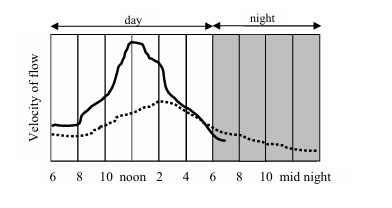
\includegraphics[width=0.7\columnwidth]{FIG/J-18.png}
\caption*{}
\label{fig:J-18}
\end{figure}

\begin{enumerate}[label=(\Alph*)]
\item The continuous line represents the trunk, and the dotted line a twig
\item The continuous line represents a twig, and the dotted line the trunk
\item The continuous line represents a root, and the dotted line a twig
\item The continuous line represents a root, and the dotted line the trunk
\end{enumerate}

\item Given below are the names of some genes/enzymes and their use in genetically modified crops. Match the two columns. \\

\textbf{Gene/enzyme \hspace{2cm} Commercial use} \\
P. Bt gene \hspace{3.2cm} i. Golden rice \\
Q. $\beta$-carotene biosynthetic genes \hspace{0.7cm} ii. insect resistance \\
R. ACC deaminase \hspace{2cm} iii. herbicide resistance \\
S. EPSP synthase \hspace{2.1cm} iv. fruit ripening

\begin{multicols}{2}
\begin{enumerate}[label=(\Alph*)]
\item P, i; Q, ii; R, iii; S, iv
\item P, ii; Q, i; R, iv; S, iii
\item P, iii; Q, i; R, ii; S, iv
\item P, ii; Q, i; R, iii; S, iv
\end{enumerate}
\end{multicols}

\item The basic tenets of the ABC model of Arabidopsis flower development are shown below along with a diagram.\\
\begin{figure}[H]
\centering
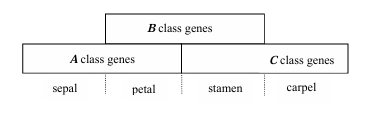
\includegraphics[width=0.7\columnwidth]{FIG/J-20.png}
\caption*{}
\label{fig:J-20}
\end{figure}
i. A class genes acting alone determine sepal identity \\
ii. A and B class genes acting together determine petal identity \\
iii. B and C class genes acting together determine stamen identity \\
iv. C class genes acting alone determine carpel identity \\
v. A and C class genes mutually inhibit each other

Which of the following organ arrangements is found in an A class mutant?

\begin{multicols}{2}
\begin{enumerate}[label=(\Alph*)]
\item sepal; petal; stamen; carpel
\item carpel; stamen; stamen; carpel
\item petal; petal; stamen; carpel
\item stamen; stamen; stamen; carpel
\end{enumerate}
\end{multicols}

\end{enumerate}

\begin{center}
\textbf{END OF QUESTION PAPER}
\end{center}
\newpage
\section*{\centering K : MICROBIOLOGY}

\noindent \textbf{ 1 -- 10 carry one mark each.}

\begin{enumerate}[label=\arabic*.]

\item Which one of the following is the most appropriate technique to determine the relatedness of two bacterial species?

\begin{multicols}{2}
\begin{enumerate}[label=(\Alph*)]
\item DNA hybridization
\item Doubling time measurement
\item Biochemical characterization
\item Plasmid profiling
\end{enumerate}
\end{multicols}

\item Which one of the following phages undergoes non-integrative lysogenic phase?

\begin{multicols}{4}
\begin{enumerate}[label=(\Alph*)]
\item $\lambda$
\item P1
\item T7
\item M13
\end{enumerate}
\end{multicols}

\item Which one of the following is NOT a part of human microbiome?

\begin{multicols}{2}
\begin{enumerate}[label=(\Alph*)]
\item Propionibacterium acnes
\item Lactobacillus casei
\item Streptococcus suis
\item Bacteroides fragilis
\end{enumerate}
\end{multicols}

\item Resident macrophages of\rule{2.5cm}{0.1pt} are called Kupffer cells.

\begin{multicols}{4}
\begin{enumerate}[label=(\Alph*)]
\item brain
\item liver
\item lung
\item kidney
\end{enumerate}
\end{multicols}

\item The enzyme responsible for generation of hypochlorous ions during phagocytosis is

\begin{multicols}{2}
\begin{enumerate}[label=(\Alph*)]
\item NADPH oxidase
\item catalase
\item myeloperoxidase
\item superoxide dismutase
\end{enumerate}
\end{multicols}

\item Teichoic acid is composed of repetitive units of

\begin{multicols}{2}
\begin{enumerate}[label=(\Alph*)]
\item keto-deoxy octanoic acid
\item glucose
\item N-acetyl glucosamine
\item glycerol
\end{enumerate}
\end{multicols}

\item Biofilm produced by bacteria is detected by

\begin{multicols}{4}
\begin{enumerate}[label=(\Alph*)]
\item Saffranin
\item Malachite green
\item Basic fuchsin
\item Congo red
\end{enumerate}
\end{multicols}

\item The precursor for the synthesis of aromatic amino acids is

\begin{multicols}{2}
\begin{enumerate}[label=(\Alph*)]
\item phosphoenolpyruvate
\item pyruvate
\item oxaloacetate
\item $\alpha$-ketoglutarate
\end{enumerate}
\end{multicols}

\item The net yield of NADH in the Embden-Meyerhof pathway in E. coli is \rule{2.5cm}{0.1pt}.

\item E. coli ribonuclease contains 124 amino acids. The number of nucleotides present in the gene encoding the protein is \rule{2.5cm}{0.1pt}.

\end{enumerate}

\vspace{0.5cm}
\noindent \textbf{ 11 -- 20 carry two marks each.}

\begin{enumerate}[label=\arabic*.,resume]

\item Which of the following infectious agents cross the blood-brain barrier?

\begin{enumerate}[label=(\Alph*)]
\item Streptococcus pneumoniae and Streptococcus pyogenes
\item Rotavirus and Streptococcus pyogenes
\item Streptococcus pneumoniae and Coxsackie virus
\item Coxsackie virus and Rotavirus
\end{enumerate}

\item At OD540nm= 0.5, which one of the following bacterial mono-dispersed cell suspensions will have (i) maximum and (ii) minimum number of cells?

\begin{enumerate}[label=(\Alph*)]
\item Mycoplasma pneumoniae and Micrococcus luteus
\item Mycoplasma pneumoniae and Bacillus subtilis
\item Micrococcus luteus and Bacillus subtilis
\item Bacillus subtilis and Escherichia coli
\end{enumerate}

\item Which one of the following enzyme combinations allows some bacteria to utilize acetate through glyoxylate pathway?

\begin{enumerate}[label=(\Alph*)]
\item Isocitrate lyase and Malate synthase
\item Isocitrate lyase and Succinyl CoA synthetase
\item Isocitrate dehydrogenase and Malate synthase
\item Isocitrate dehydrogenase and Succinyl CoA synthetase
\end{enumerate}

\item The decimal reduction time (D121) for Clostridium botulinum spores is 0.2 min. The time required to reduce the spore count from 10$^{12}$ to one spore at 121$^\circ$C is \rule{2.5cm}{0.1pt} minutes.

\item E. coli requires three genes, galK (kinase), galT (transacetylase) and galE (epimerase) to utilize galactose. If there is a mutation in any one of these genes, the mutant cannot utilize galactose. Which one of the following combinations of merodiploids will support the growth of mutants on galactose?

\begin{enumerate}[label=(\Alph*)]
\item galK$^+$galT$^+$galE$^-$/galK$^-$galT$^+$galE$^-$ 
\item galK$^-$galT$^+$galE$^-$/galK$^+$galT$^-$galE$^+$ 
\item galK$^+$galT$^-$galE$^-$/galK$^-$galT$^-$galE$^+$
\item galK$^+$galT$^+$galE$^-$/galK$^+$galT$^-$galE$^+$
\end{enumerate}

\item Nitrogenase reduces N$_2$ to NH$_3$. Metal co-factors required for this activity are

\begin{multicols}{4}
\begin{enumerate}[label=(\Alph*)]
\item Fe and Cu
\item Mo and Fe
\item Mo and Mn
\item Cu and Mn
\end{enumerate}
\end{multicols}

\item If a bacterial cell contains 5,000 genes and if the average mutation frequency per gene is $2 \times 10^{-4}$ per generation, the average number of new mutations per generation is \rule{2.5cm}{0.1pt}.

\item The growth profile of \textit{E. coli} on glucose plus lactose is shown below. The specific growth rate of the second exponential phase is \rule{2.5cm}{0.1pt} h$^{-1}$.

\begin{figure}[H]
\centering
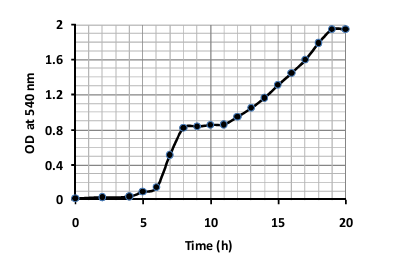
\includegraphics[width=0.7\columnwidth]{FIG/K-18.png}
\caption*{}
\label{fig:K-18}
\end{figure}

\item Match the cell structure components given in Group I with appropriate functions from Group II.

\textbf{Group I} \hspace{2cm} \textbf{Group II} \\
(P) Cell membrane \hspace{2.5cm} (I) Nutrient transport \\
(Q) Purple membrane \hspace{2.5cm} (II) Photosynthesis \\
(R) Cisternae \hspace{3.1cm} (III) Active transport \\
(S) Outer membrane \hspace{2.5cm} (IV) Protein glycosylation \\
\hspace{2.4cm} \hspace{3cm} (V) Light-driven proton transport

\begin{multicols}{2}
\begin{enumerate}[label=(\Alph*)]
\item P-I, Q-V, R-II, S-III
\item P-I, Q-II, R-IV, S-III
\item P-III, Q-II, R-V, S-I
\item P-III, Q-V, R-IV, S-I
\end{enumerate}
\end{multicols}

\item Match the antibiotics given in Group I with appropriate targets from Group II.

\textbf{Group I} \hspace{2cm} \textbf{Group II} \\
(P) Nalidixic acid \hspace{2.5cm} (I) RNA polymerase \\
(Q) Tetracycline \hspace{3cm} (II) DNA gyrase \\
(R) Erythromycin \hspace{2.3cm} (III) DNA polymerase \\
(S) Rifampin \hspace{3.2cm} (IV) 50S ribosomal subunit \\
\hspace{3.3cm} \hspace{3cm} (V) Aminoacyl tRNA

\begin{multicols}{2}
\begin{enumerate}[label=(\Alph*)]
\item P-III, Q-IV, R-V, S-I
\item P-V, Q-I, R-IV, S-II
\item P-II, Q-V, R-IV, S-I
\item P-II, Q-V, R-I, S-IV
\end{enumerate}
\end{multicols}

\end{enumerate}

\begin{center}
\textbf{END OF QUESTION PAPER}
\end{center}
\newpage
\section*{\centering L : ZOOLOGY}

\noindent \textbf{ 1 -- 10 carry one mark each.}

\begin{enumerate}[label=\arabic*.]

\item Acorn worms (Saccoglossus sp.) belong to which ONE of the following Phyla?

\begin{multicols}{4}
\begin{enumerate}[label=(\Alph*)]
\item Platyhelminthes
\item Achelminthes
\item Hemichordata (Chordata)
\item Annelida
\end{enumerate}
\end{multicols}

\item A population of Bees develops resistance to pesticides and the trait gets fixed within a few generations. This is an example of

\begin{multicols}{4}
\begin{enumerate}[label=(\Alph*)]
\item macroevolution
\item disruptive selection
\item stabilizing selection
\item microevolution
\end{enumerate}
\end{multicols}

\item The nature of the polymorphic DNA fragment used for mapping is

\begin{multicols}{4}
\begin{enumerate}[label=(\Alph*)]
\item dominant
\item partial dominant
\item co-dominant
\item recessive
\end{enumerate}
\end{multicols}

\item The sex of a Drosophila melanogaster, which has 4 copies of X-chromosomes and 4 sets of autosomes will be

\begin{multicols}{4}
\begin{enumerate}[label=(\Alph*)]
\item female
\item male
\item metafemale
\item metamale
\end{enumerate}
\end{multicols}

\item Which of the following cations are found in higher concentration in extracellular fluid as compared to intracellular fluid in animals?

\begin{multicols}{4}
\begin{enumerate}[label=(\Alph*)]
\item Na$^+$ and Ca$^{++}$
\item K$^+$ and Ca$^{++}$
\item K$^+$ and Mg$^{++}$
\item Na$^+$ and Mg$^{++}$
\end{enumerate}
\end{multicols}

\item Detoxification of alcohol occurs in liver cells where peroxisomal enzymes remove hydrogen from it, which is

\begin{multicols}{2}
\begin{enumerate}[label=(\Alph*)]
\item combined with water molecules to generate hydrogen peroxide
\item used to break down hydrogen peroxide
\item transferred to the mitochondria
\item transferred to oxygen molecules to generate hydrogen peroxide
\end{enumerate}
\end{multicols}

\item When cells are treated with cyanide, which ONE of the following organelles will have the highest level of cyanide inside?

\begin{multicols}{2}
\begin{enumerate}[label=(\Alph*)]
\item Mitochondria
\item Peroxisomes
\item Lysosomes
\item Endoplasmic reticulum
\end{enumerate}
\end{multicols}

\item Toxoplasmosis in humans is caused by Toxoplasma gondii, an obligate intracellular parasite with two different life cycles, sexual and asexual.  The sexual cycle occurs in which ONE of the following definitive hosts?

\begin{multicols}{4}
\begin{enumerate}[label=(\Alph*)]
\item Dog
\item Cat
\item Rat
\item Human
\end{enumerate}
\end{multicols}

\item Which ONE of the following is often a life-threatening systemic inflammatory response?

\begin{multicols}{2}
\begin{enumerate}[label=(\Alph*)]
\item Tuberculosis
\item Lupus erythematosus
\item Septic shock
\item Hypertension
\end{enumerate}
\end{multicols}

\item During the gastrulation stage of amphibian development, ectoderm formation takes place by the expansion of epithelial cell sheet over mesodermal cells. This type of cell movement is termed as

\begin{multicols}{4}
\begin{enumerate}[label=(\Alph*)]
\item ingression
\item epiboly
\item involution
\item delamination
\end{enumerate}
\end{multicols}

\end{enumerate}

\vspace{0.5cm}
\noindent \textbf{ 11 -- 20 carry two marks each.}

\begin{enumerate}[label=\arabic*.,resume]

\item In a population, 600 individuals have MM blood group, 300 have MN blood group and 100 have NN blood group. What will be the frequencies of M and N alleles in this population?

\begin{multicols}{2}
\begin{enumerate}[label=(\Alph*)]
\item M 0.75 and N 0.25
\item M 0.65 and N 0.35
\item M 0.85 and N 0.15
\item M 0.55 and N 0.45
\end{enumerate}
\end{multicols}

\item The molecules, hexanoic acid, lysine, histidine and glucose, each contain 6 carbon atoms, but have completely different properties due to the presence of different functional groups.  Which ONE of these molecules has a high calorific value?

\begin{multicols}{4}
\begin{enumerate}[label=(\Alph*)]
\item Lysine
\item Hexanoic acid
\item Glucose
\item Histidine
\end{enumerate}
\end{multicols}

\item The primary function of polysaccharides attached to glycoproteins in the animal cell membrane is to

\begin{enumerate}[label=(\Alph*)]
\item facilitate diffusion of molecules down their concentration gradients
\item maintain membrane fluidity at low temperatures
\item maintain the integrity of a fluid mosaic membrane
\item mediate cell-to-cell recognition
\end{enumerate}
\item Which ONE of the following mechanisms is used to coordinate the expression of multiple, related genes in eukaryotic cells?

\begin{enumerate}[label=(\Alph*)]
\item Environmental signals enter the cell and bind directly to promoters
\item Genes share a common intragenic sequence, and allow several activators to turn on their transcription, regardless of location
\item Genes are organized into large operons, allowing them to be transcribed as a single unit
\item Genes are organized into clusters, with local chromatin structures influencing the expression of all the clustered genes at once
\end{enumerate}

\item In an experiment involving development of 64-cell stage sea urchin, an isolated animal hemisphere was combined with isolated micromeres. Which ONE of the following will be the resulting structure?

\begin{multicols}{2}
\begin{enumerate}[label=(\Alph*)]
\item A ball of ectomesodermal cells
\item A ciliated ball of ectodermal cells
\item A recognizable pluteus larva
\item A ball of endodermal cells
\end{enumerate}
\end{multicols}

\item Glycoprotein hormones, hCG and eCG, are synthesized in women and mares respectively, during pregnancy. Both of these chorionic gonadotropin hormones
\begin{enumerate}[label=(\Alph*)]
\item have only LH-like activity in their respective species
\item have only FSH-like activity in other species
\item are biologically inactive in other species
\item are routinely employed to promote final stages of follicular maturation, ovulation and to treat infertility in women
\end{enumerate}

\item Entamoeba histolytica is an intestinal parasite that causes dysentery in humans. This parasite resides in the isotonic environment of intestine and other tissues in the human body and does not possess contractile vacuoles. If this parasite is placed in fresh water, it will

\begin{enumerate}[label=(\Alph*)]
\item survive for long time, until they re-enter the host environment
\item die due to hypoosmotic shock
\item not survive in water as they require high salt content
\item die due to hyperosmotic shock
\end{enumerate}

\item In an experiment involving Drosophila development, a large amount of purified bicoid mRNA was injected into the posterior end of a wild-type embryo, the resulting developing embryo will have

\begin{enumerate}[label=(\Alph*)]
\item normal development with one each of head, thorax and abdomen
\item head in the middle with two thoraces and two abdomens
\item a head with two thoraces and an abdomen
\item two heads and two thoraces with an abdomen segment in the middle
\end{enumerate}

\item The migratory desert locust, Schistocerca gregaria, exists in two mutually exclusive forms: a short-winged, uniformly colored, solitary insect and a long-winged, brightly colored, gregarious morph. These phenotypes depend on crowding. Such phenotypic plasticity is called

\begin{multicols}{4}
\begin{enumerate}[label=(\Alph*)]
\item reaction norm
\item polyphenism
\item Batesian mimicry
\item polymorphism
\end{enumerate}
\end{multicols}

\item Given below is the list of animals and their respective characteristics.

\begin{tabular}{rl}
I. & Sea anemone \\
II. & Bluefly \\
III. & Starfish \\
IV. & Sponge
\end{tabular}
\quad
\begin{tabular}{rl}
i. & Three pairs of jointed legs \\
ii. & Diploblastic acoelomate \\
iii. & Collar cells \\
iv. & Tube feet
\end{tabular}

Which ONE of the following represents the correct match?

\begin{multicols}{2}
\begin{enumerate}[label=(\Alph*)]
\item I-iv; II-i; III-ii; IV-iii
\item I-iii; II-i; III-iv; IV-ii
\item I-ii; II-i; III-iv; IV-iii
\item I-ii; II-i; III-iii; IV-iv
\end{enumerate}
\end{multicols}

\end{enumerate}

\begin{center}
\textbf{END OF QUESTION PAPER}
\end{center}
\newpage
\section*{\centering M : FOOD TECHNOLOGY}

\noindent \textbf{ 1 -- 10 carry one mark each.}

\begin{enumerate}[label=\arabic*.]

\item Bread staling is caused by

\begin{multicols}{4}
\begin{enumerate}[label=(\Alph*)]
\item Caramelisation
\item Gelatinisation
\item Retrogradation
\item Aggregation
\end{enumerate}
\end{multicols}

\item The grades of tea in the increasing order of their leaf size are \rule{1.5cm}{0.1pt}, \rule{1.5cm}{0.1pt}and\rule{1.5cm}{0.1pt} .

\begin{multicols}{2}
\begin{enumerate}[label=(\Alph*)]
\item Souchang, pekoe and orange pekoe
\item Pekoe, souchang and orange pekoe
\item Orange pekoe, souchang, and pekoe
\item Orange pekoe, pekoe, and souchang
\end{enumerate}
\end{multicols}

\item Fruit juice is being pasteurized in a tubular heat exchanger. The retention time in holding tube of 0.2 m$^2$ cross sectional area is 3 seconds. If the flow rate of juice is 0.4 m$^3$ s$^{-1}$, the length of the holding tube in m, is \rule{2.5cm}{0.1pt}.

\item The oil, which experiences flavor reversion even at the lower peroxide value is

\begin{multicols}{4}
\begin{enumerate}[label=(\Alph*)]
\item Mustard
\item Soybean
\item Palm
\item Sesame
\end{enumerate}
\end{multicols}

\item 80 kg of wheat containing 10 kg of moisture has been dried to a moisture content of 8\% wet basis in 3 hours under constant rate period of drying. The drying rate in kg h$^{-1}$ is \rule{2.5cm}{0.1pt}.

\item The rate of cream separation in a disc bowl centrifuge can be increased by

\begin{multicols}{2}
\begin{enumerate}[label=(\Alph*)]
\item Increasing the size of the bowl
\item Lower viscosity of fluid
\item Increasing RPM of the bowl
\item All of these
\end{enumerate}
\end{multicols}

\item Rigor mortis is caused due to

\begin{enumerate}[label=(\Alph*)]
\item Unavailability of ATP which is necessary to break the link between actin and myosin
\item Rupturing of tissue due to unavailability of oxygen
\item Decrease in body temperature
\item Breakage of rigid protein molecules in sarcoplasm
\end{enumerate}

\item Oxygen is permeating through an EVOH film of thickness ‘t’ and solubility coefficient ‘S’. If diffusivity of oxygen through the film is ‘D’, then permeability of oxygen through the film will be

\begin{multicols}{4}
\begin{enumerate}[label=(\Alph*)]
\item $D/t$
\item $D/S$
\item $D \times S$
\item $S/D$
\end{enumerate}
\end{multicols}

\item Condensing steam is used to heat vegetable oil in a double pipe co-current heat exchanger. If the inlet and outlet temperature of steam are $T_{hi}$ and $T_{ho}$, and for vegetable oil $T_{ci}$ and $T_{co}$ respectively, the log mean temperature difference ($\Delta T_{LM}$) will be

\begin{multicols}{4}
\begin{enumerate}[label=(\Alph*)]
\item $\ln \frac{T_{hi} - T_{co}}{T_{hi} - T_{ci}}$
\item $\frac{(T_{ho} - T_{co}) - (T_{hi} - T_{ci})}{\ln \frac{T_{ho} - T_{co}}{T_{hi} - T_{ci}}}$
\item $\ln \frac{T_{hi} - T_{co}}{T_{ho} - T_{ci}}$
\item $\ln \frac{T_{co} - T_{ci}}{T_{hi} - T_{co}}$
\end{enumerate}
\end{multicols}

\item To produce Blue veined cheese, the curd is inoculated with strains of

\begin{multicols}{2}
\begin{enumerate}[label=(\Alph*)]
\item Propionibacterium shermanii
\item Penicilium roqueforti
\item Pencilium camemberti
\item Brevibacterium linens
\end{enumerate}
\end{multicols}

\end{enumerate}

\vspace{0.5cm}
\noindent \textbf{ 11 -- 20 carry two marks each.}

\begin{enumerate}[label=\arabic*.,resume]

\item Match the food spoilage organisms given in Column I with the associated foods given in Column II \\

\textbf{Column I} \hspace{4cm} \textbf{Column II} \\[6pt]

\begin{tabular}{p{6cm} p{8cm}}
P. Clostridium botulinum     & 1. Fish \\
Q. Salmonella spp.           & 2. Cooked starch foods \\
R. Vibrio parahaemolyticus   & 3. Meat, egg and poultry \\
S. Bacillus cereus           & 4. Canned foods \\
\end{tabular}


\begin{multicols}{2}
\begin{enumerate}[label=(\Alph*)]
\item P-4, Q-3, R-1, S-2
\item P-3, Q-4, R-2, S-1
\item P-2, Q-1, R-3, S-4
\item P-4, Q-3, R-2, S-1
\end{enumerate}
\end{multicols}

\item Fluid is flowing inside a pipe of radius `R` in fully developed laminar flow. If the velocity of the fluid at the centre at a distance `L` is $v_{\max}$, velocity at radial distance of $\frac{3}{4} R$ will be \rule{1cm}{0.1pt} times $v_{\max}$

\begin{multicols}{4}
\begin{enumerate}[label=(\Alph*)]
\item $\frac{9}{16}$
\item $\frac{7}{16}$
\item $\frac{16}{9}$
\item $\frac{16}{7}$
\end{enumerate}
\end{multicols}

\item The amount of sugar to be added (kg) to 40 kg of mango pulp to increase its total soluble solids from 20\% wt. to 65\% wt. is \rule{2.5cm}{0.1pt}.

\item Assertion: Acidulates are added in soft drinks to provide a buffering action.\\
Reason: Buffers tend to prevent changes in pH and prevent excessive tartness.\\
Choose the correct answer from the following

\begin{enumerate}[label=(\Alph*)]
\item Both assertion and reason are true and reason is the correct explanation of assertion
\item Both assertion and reason are true but reason is not the correct explanation of assertion
\item Assertion is true but reason is false
\item Both assertion and reason are false
\end{enumerate}

\item The D121 and Z values for C. botulinum spores in canned food are 0.2 min and 10$^\circ$C, respectively. Total time required in min, to reduce the spores from 10$^2$ to 10$^{-6}$ at 111$^\circ$C is \rule{2.5cm}{0.1pt}.

\item In a typical Psychrometric Chart shown below, the processes OP, OQ and OR related to air water vapor mixture are \rule{1.5cm}{0.1pt}, \rule{1.5cm}{0.1pt}and \rule{1.5cm}{0.1pt}.

\begin{figure}[H]
\centering
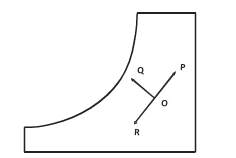
\includegraphics[width=0.7\columnwidth]{FIG/M-16.png}
\caption*{}
\label{fig:M-16}
\end{figure}

\begin{enumerate}[label=(\Alph*)]
\item Cooling \& dehumidification, cooling \& humidification, heating \& humidification
\item Cooling \& dehumidification, heating \& humidification, drying
\item Heating \& humidification, cooling \& humidification, cooling \& dehumidification
\item Heating \& humidification, cooling \& dehumidification, drying
\end{enumerate}

\item Match the enzymes in Column I with their functions in Column II \\

\textbf{Column I} \hspace{4cm} \textbf{Column II} \\[6pt]

\begin{tabular}{p{6cm} p{9cm}}
P. Amylase      & 1. Conversion of sucrose to glucose and fructose \\
Q. Invertase    & 2. Softening of dough \\
R. Phosphatase  & 3. Effectiveness of pasteurization \\
S. Protease     & 4. Conversion of starch to maltose \\
\end{tabular}


\begin{multicols}{2}
\begin{enumerate}[label=(\Alph*)]
\item P-1, Q-2, R-3, S-4
\item P-4, Q-1, R-3, S-2
\item P-1, Q-4, R-2, S-3
\item P-2, Q-4, R-3, S-1
\end{enumerate}
\end{multicols}

\item Match the terms in Column I with their most appropriate description in Column II \\

\textbf{Column I} \hspace{4cm} \textbf{Column II} \\[6pt]

\begin{tabular}{p{6cm} p{8cm}}
P. Enrichment of two plant sources & 1. Overcome the deficiency of nutrients by mixing \\
Q. Fortification synthetic source & 2. Overcome the deficiency of nutrients from a synthetic source \\
R. Supplementation processing & 3. Restoration of nutrients which are lost during processing \\
S. Complementation originally present & 4. Addition of nutrients which may or may not be originally present \\
\end{tabular}


\begin{multicols}{2}
\begin{enumerate}[label=(\Alph*)]
\item P-3, Q-4, R-2, S-1
\item P-4, Q-3, R-1, S-2
\item P-1, Q-2, R-3, S-4
\item P-2, Q-3, R-1, S-4
\end{enumerate}
\end{multicols}

\item Match the products in Column I with their Original Phase in Column II \\

\textbf{Column I} \hspace{4cm} \textbf{Column II} \\[6pt]

\begin{tabular}{p{6cm} p{8cm}}
P. Milk    & 1. Colloidal \\
Q. Butter  & 2. Solution \\
R. Lactose & 3. Water in oil emulsion \\
S. Casein  & 4. Oil in water emulsion \\
\end{tabular}

\begin{multicols}{2}
\begin{enumerate}[label=(\Alph*)]
\item P-3, Q-4, R-1, S-2
\item P-3, Q-4, R-2, S-1
\item P-4, Q-3, R-2, S-1
\item P-4, Q-3, R-1, S-2
\end{enumerate}
\end{multicols}

\item Assertion: Presence of low sulphur containing amino acids makes casein in milk to boil, sterilize and concentrate without coagulation even at higher temperatures. \\
Reason: This is due to the restricted formation of di-sulphide bonds resulting in increased stability. \\
Choose the correct answer from the following

\begin{enumerate}[label=(\Alph*)]
\item Both assertion and reason are true and reason is the correct explanation of assertion
\item Both assertion and reason are true but reason is not the correct explanation of assertion
\item Both assertion and reason are false
\item Assertion is true but reason is false
\end{enumerate}
\end{enumerate}

\begin{center}
\textbf{END OF QUESTION PAPER}
\end{center}

\end{document}
